\chapter{RAISE 动态路由与弱网补偿}

边缘推理回答“当前能够看出什么”，RAISE 则回答“下一步应把有限的分析资源用在哪里”。它先评估事件的分析价值，再结合系统当时是否适合调用云端，最终在 \texttt{LOCAL}、\texttt{CLOUD} 和 \texttt{DEFER} 之间选择动作。

\section{联合感知的决策输入}
RAISE（Risk-Aware, uncertainty-calibrated, Intent-constrained, Self-adaptive Edge-cloud routing）不是只看一个置信度阈值。其输入由事件侧和系统侧两组信号构成。

\begin{table}[htbp]
  \centering
  \small
  \caption{RAISE 的联合感知因素}
  \label{tab:raise-inputs}
  \begin{tabularx}{\textwidth}{>{\bfseries}p{0.18\textwidth} p{0.28\textwidth} X}
    \toprule
    信号类别 & 代表因素 & 对决策的影响 \\
    \midrule
    事件风险 & 严重度、影响范围、推理路径风险 & 风险越高，越需要更强诊断与更高处理优先级 \\
    认知不确定性 & 置信度校准、不确定性、模板新颖度、历史边云分歧 & 边缘越没有把握，云端复核价值通常越高 \\
    运行条件 & 网络状态、云端健康、队列压力、调用预算与限流 & 条件恶化时提高即时上云门槛，避免主链拥塞 \\
    运维意图 & 禁止上云、强制本地、强制云端等硬策略 & 明确的隐私与生产规则优先于软评分 \\
    \bottomrule
  \end{tabularx}
\end{table}

事件分数描述“这条事件是否值得获得更强能力”，动态门槛描述“系统此刻能承担多少云端任务”。两者分开后，同一类日志可以在网络畅通与网络受限时得到不同动作，同时保持可解释的原因记录。

\section{价值评分与系统成本建模}
对时刻 $t$ 到达的事件 $e_t$，RAISE 将事件本身的分析价值、云端可能带来的新增收益和当前系统成本组合为
\begin{equation}
  S_t = \beta_v V(e_t) + \beta_g G(e_t) - \beta_k K(e_t,s_t),
  \label{eq:raise-score-v03}
\end{equation}
其中，$V(e_t)$ 由严重度、不确定性、模板新颖度、历史边云分歧、影响范围和推理路径风险构成；$G(e_t)$ 表示云端相对于当前边缘结果可能补充的诊断信息；$K(e_t,s_t)$ 表示调用费用、处理时延、网络压力、队列压力、预算占用和隐私风险等代价。

式\eqref{eq:raise-score-v03}可以直观理解为“事件值得深入分析的程度，加上云端可能带来的认知增益，再减去此刻使用云端的综合代价”。各特征在进入评分前完成归一化，使风险、置信度、字节量和系统压力等不同量纲能够在统一空间中比较。该结构也保留了明确的工程解释：事件侧因素决定是否有必要获得更强能力，状态侧因素决定此时调用这项能力是否划算。

\section{动态门槛与容量调节}
系统门槛定义为
\begin{equation}
  \Theta_t = \Theta_0 + \alpha_q Q_t + \alpha_b B_t + \alpha_n N_t - \alpha_a A_t,
  \label{eq:raise-threshold-v03}
\end{equation}
其中，$Q_t$、$B_t$、$N_t$ 和 $A_t$ 分别表示队列压力、预算压力、网络压力和审计采样不足程度。队列拥塞、预算紧张或网络条件恶化时，门槛随之提高，系统将更多事件保留在边缘或延期处理；近期缺少云端复核样本时，审计项可以适度降低门槛，为边缘结论保留必要的抽样校验。

动态门槛使 RAISE 不必为所有部署环境使用同一个固定置信度阈值。在输入内容相同的情况下，网络畅通、队列空闲且预算充足时，系统可以主动获取更多云端增益；资源紧张时则优先保障现场主链。门槛、压力项和最终动作随事件共同保存，使容量调节不是不可见的内部行为，而是可以被运行界面解释和复盘的决策依据。

\section{三动作在线路由算法}
\begin{algorithm}[htbp]
  \caption{RAISE 三动作在线路由}
  \label{alg:raise-v03}
  \KwInput{事件 $e_t$，边缘结果，系统状态 $s_t$，运维策略}
  \KwOutput{$\texttt{LOCAL}$、$\texttt{CLOUD}$ 或 $\texttt{DEFER}$}
  执行禁止上云、强制本地和强制云端等硬约束\;
  计算事件分数 $S_t$ 与动态门槛 $\Theta_t$\;
  \eIf{$S_t < \Theta_t$}{
    \KwRet{$\texttt{LOCAL}$}\;
  }{
    \eIf{网络、云端健康、预算和限流条件允许}{
      \KwRet{$\texttt{CLOUD}$}\;
    }{
      将事件持久化到优先级 Outbox\;
      \KwRet{$\texttt{DEFER}$}\;
    }
  }
\end{algorithm}

算法\ref{alg:raise-v03}首先执行运维硬约束，再计算软评分。这样的顺序保证禁止上云、数据边界和生产安全策略不会被在线模型或统计分数覆盖。动作产生后，路由器保存事件分数、动态门槛、关键特征、动作原因和系统状态快照，既为管理端提供解释，也为后续策略评估和重放审计提供依据。

\section{反馈信号与自适应衔接}
Cloud Gateway 会依据云端纠正、根因与建议完整性、高风险确认、置信度变化、延迟和 Token 使用构造复合反馈：
\begin{equation}
  r=\operatorname{clip}_{[-1,1]}\!\left(
  0.35D+0.30A+0.20H+0.15\Delta c-0.10L-0.05T
  \right),
  \label{eq:cloud-reward-v03}
\end{equation}
其中，$D$ 表示云端是否有效纠正边缘判断，$A$ 表示是否同时提供根因与建议，$H$ 表示是否确认高风险事件，$\Delta c$ 表示正向置信度变化，$L$ 和 $T$ 分别是归一化后的时延与 Token 惩罚。该反馈把诊断增益和资源成本放入同一信号，为模板纠错统计、探索状态和 GainModel 更新提供输入。

Router 当前会依据首个匹配条件对反馈重新归类，并更新模板统计、探索状态和 GainModel 快照。现有离散归类可能覆盖 Gateway 生成的复合值，已学习增益也尚未直接参与式\eqref{eq:raise-score-v03}。因此，当前反馈链首先承担结果记录、统计更新和后续学习数据积累；进一步自适应需要统一两阶段 Reward 语义，再通过灰度发布、状态快照和可回滚机制安全接入在线评分。

\section{三动作语义}
\begin{table}[htbp]
  \centering
  \small
  \caption{RAISE 三种动作的业务含义}
  \label{tab:raise-actions}
  \begin{tabularx}{\textwidth}{>{\ttfamily\bfseries}p{0.16\textwidth} X X}
    \toprule
    \normalfont\bfseries 动作 & \textbf{触发语义} & \textbf{后续处理} \\
    \midrule
    LOCAL & 边缘已有足够信息，或策略要求留在本地 & 保存并发布边缘判断，供现场系统继续消费 \\
    CLOUD & 事件值得上云，且网络、预算、健康与限流条件允许 & 立即进入云端请求流，聚合上下文后深诊 \\
    DEFER & 事件值得上云，但当前发送条件不满足 & 写入持久化 Outbox，后续按优先级重试 \\
    \bottomrule
  \end{tabularx}
\end{table}

\texttt{DEFER} 的关键意义是把“值得上云”与“现在能够发送”解耦。没有该动作时，断网中的高价值事件只能被迫留在本地或直接失败；引入延期后，实时主链继续产出边缘结果，后续深诊机会则由独立队列保存。

\section{路由运行状态}
\begin{figure}[htbp]
  \centering
  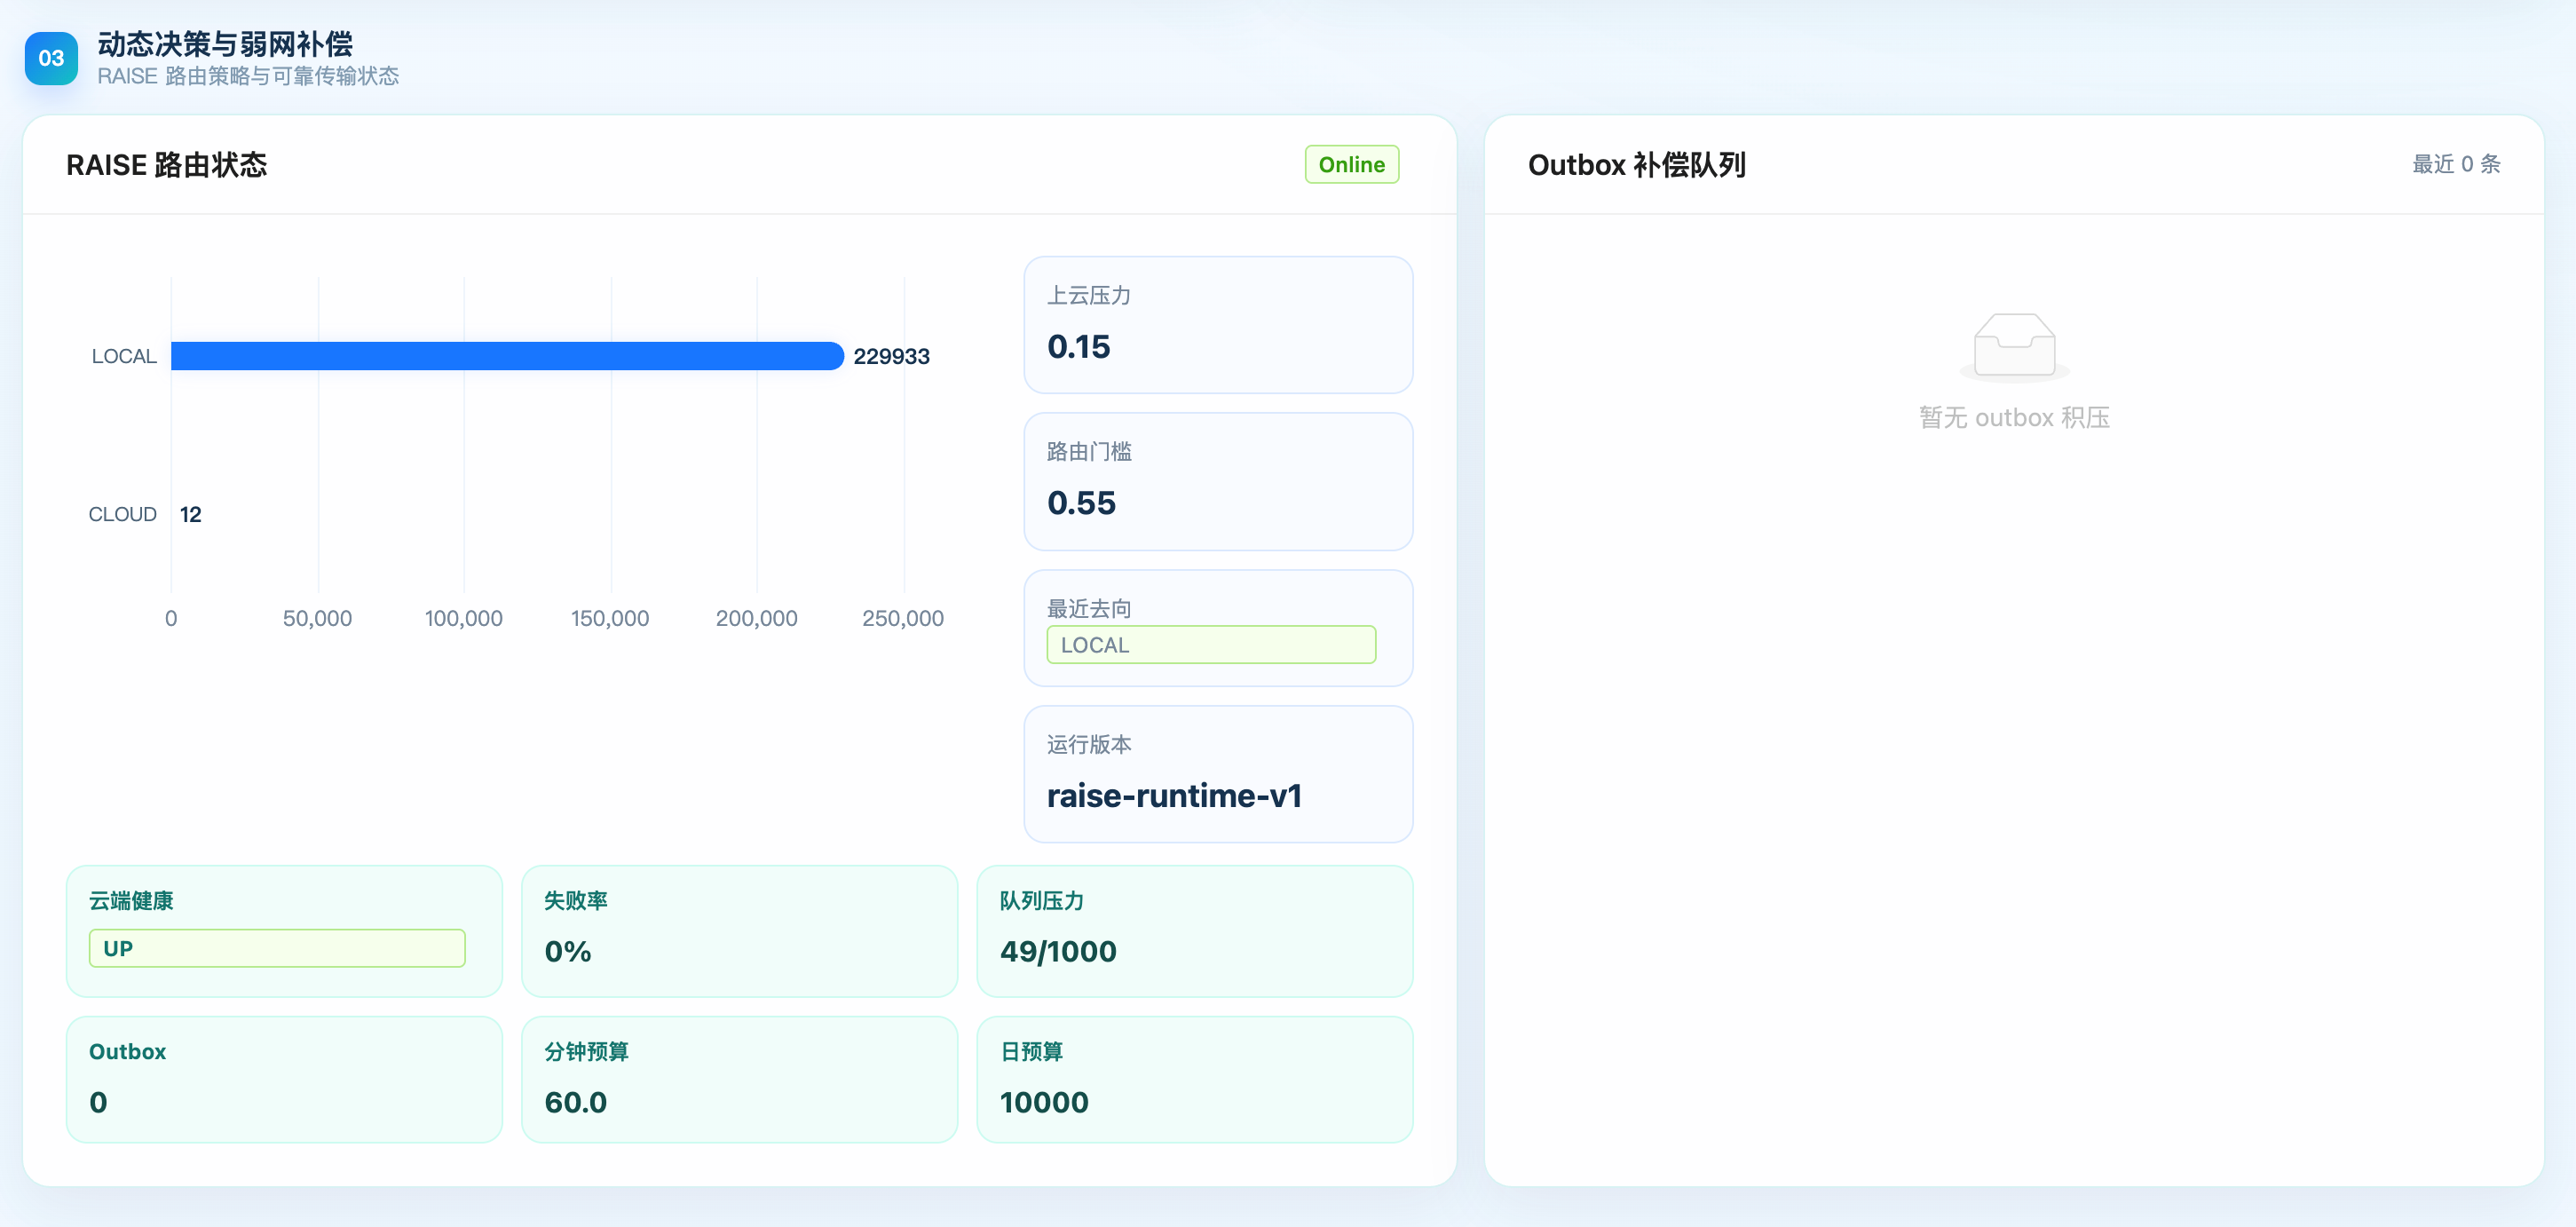
\includegraphics[width=0.98\textwidth]{figures/s-04a-raise-routing-status-overview.png}
  \caption{RAISE 路由状态、系统压力与 Outbox 的统一展示}
  \label{fig:raise-routing-overview}
\end{figure}

\cref{fig:raise-routing-overview}集中展示 \texttt{LOCAL/CLOUD} 累计数量、上云压力、动态门槛、最近动作、云端健康、队列压力、预算与 Outbox。它帮助运维人员判断系统当前如何分流，以及外部条件是否正在改变门槛。该画面是运行窗口的聚合状态；Outbox 为空只说明截图时没有积压，不能据此推断弱网恢复速度或重试成功率。

\section{Outbox 优先补传与死信处理}
当 RAISE 输出 \texttt{DEFER} 时，事件写入 MySQL \texttt{cloud\_outbox}。replayer 周期读取到期记录，多实例通过条件更新抢占任务；失败后按照退避策略重试，超过次数限制的记录进入 DLQ，供运维人员检查。到期任务按照 RAISE 分数降序，再按截止时间与创建时间排序，使更高风险、更紧迫的事件优先获得发送机会。

\begin{figure}[htbp]
  \centering
  \begin{tikzpicture}[
    node distance=11mm and 12mm,
    state/.style={draw=CoTriageNavy,rounded corners=1.2mm,minimum width=24mm,minimum height=10mm,fill=CoTriageGray,font=\sffamily\small\bfseries,text=CoTriageNavy,align=center},
    terminal/.style={state,draw=CoTriageCyan,fill=CoTriageCyan!8},
    failed/.style={state,draw=CoTriageRed,fill=CoTriageRed!7,text=CoTriageRed},
    flow/.style={-{Stealth[length=2.5mm]},thick,draw=CoTriageCyan},
    retry/.style={-{Stealth[length=2.5mm]},thick,dashed,draw=CoTriageOrange}
  ]
    \node[state] (pending) {PENDING\\等待到期};
    \node[state,right=of pending] (sending) {SENDING\\条件抢占};
    \node[terminal,right=of sending] (sent) {SENT\\已发布请求};
    \node[state,below=of sending] (retrying) {RETRY\\退避重试};
    \node[failed,right=of retrying] (dlq) {DLQ\\人工检查};
    \draw[flow] (pending) -- node[above,font=\footnotesize]{按优先级读取} (sending);
    \draw[flow] (sending) -- node[above,font=\footnotesize]{发布成功} (sent);
    \draw[retry] (sending) -- node[right,font=\footnotesize]{失败} (retrying);
    \draw[retry] (retrying.west) -| node[pos=0.25,below,font=\footnotesize]{未超限} (pending.south);
    \draw[retry] (retrying) -- node[above,font=\footnotesize]{超过上限} (dlq);
  \end{tikzpicture}
  \caption{Outbox 延期、重试与死信状态流}
  \label{fig:outbox-state}
\end{figure}

当前实现中的 \texttt{SENT} 表示请求已经发布到云端请求流，并不等同于云端诊断已经完成；replayer 采用周期扫描，也未以网络恢复事件直接触发。这一边界使运行状态的解释更加准确，并为后续增加云端完成确认和健康门控保留了清晰接口。

\section{运维硬策略与可解释性}
禁止上云、强制本地和强制云端等策略先于软评分执行，防止模型覆盖隐私、安全和生产要求。每次路由同时保留动作、原因、分数、门槛与系统快照，使管理员既能查看“去了哪里”，也能追溯“当时为什么这样决定”。
